\documentclass[12pt,a4paper]{article}
\usepackage[utf8]{vietnam}
\usepackage{amsmath,amssymb}
\usepackage{geometry}
\geometry{top=1.5cm,bottom=1.2cm,left=1.4cm,right=1.4cm,headheight=28pt,headsep=12pt,footskip=18pt}
\usepackage{tikz}
\usepackage{xcolor}
\usepackage{enumerate}
\usepackage{graphicx}
\usepackage[version=4]{mhchem}
\usepackage{fancyhdr}
\usepackage{ex_test}

\renewcommand{\baselinestretch}{0.96}
\setlength{\parskip}{0pt}

\definecolor{hfRed}{RGB}{211,47,47}
\definecolor{hfGreen}{RGB}{139,195,144}

\pagestyle{fancy}
\fancyhf{}
\fancyhead[L]{\small\itshape\color{hfRed} Tài liệu lưu hành nội bộ}
\fancyhead[R]{\small\itshape\color{hfRed} Thầy \textbf{TRẦN VĂN THẠNH} - 0777.470.803}
\renewcommand{\headrulewidth}{0.8pt}
\renewcommand{\headrule}{\hbox to\headwidth{\color{hfGreen}\leaders\hrule height \headrulewidth\hfill}}

\fancyfoot[L]{\small\itshape\color{hfRed} CS1: 6/15 Nguyễn Hoàng, P. Kim Long, TP Huế \quad|\quad CS2: 24 Đặng Thái Thân, TP Huế}
\fancyfoot[R]{\small\bfseries\color{hfRed} Trang \thepage}
\renewcommand{\footrulewidth}{0.8pt}
\renewcommand{\footrule}{\hbox to\headwidth{\color{hfGreen}\leaders\hrule height \footrulewidth\hfill}}

\fancypagestyle{firstpage}{
  \fancyhf{}
  \renewcommand{\headrulewidth}{0pt}
  \fancyfoot[L]{\small\itshape\color{hfRed} CS1: 6/15 Nguyễn Hoàng, P. Kim Long, TP Huế \quad|\quad CS2: 24 Đặng Thái Thân, TP Huế}
  \fancyfoot[R]{\small\bfseries\color{hfRed} Trang \thepage}
  \renewcommand{\footrulewidth}{0.8pt}
  \renewcommand{\footrule}{\hbox to\headwidth{\color{hfGreen}\leaders\hrule height \footrulewidth\hfill}}
}

\begin{document}
\thispagestyle{firstpage}

\noindent
\begin{minipage}[t]{0.44\textwidth}
	\centering\fontsize{10pt}{12pt}\selectfont
	\textbf{SỞ GIÁO DỤC VÀ ĐÀO TẠO THỪA THIÊN HUẾ}\\
	\textbf{ĐỀ CHÍNH THỨC}\\
	\textit{(Đề thi có 04 trang)}
\end{minipage}\hfill
\begin{minipage}[t]{0.54\textwidth}
	\centering\fontsize{10.5pt}{13pt}\selectfont
	\textbf{ĐỀ KIỂM TRA ĐỊNH KỲ CHƯƠNG 6}\\
	\textbf{(HỢP CHẤT CARBONYL - CARBOXYLIC ACID)}\\
	\textbf{MÔN: HOÁ HỌC - LỚP 11}\\
	\textit{Thời gian làm bài: 50 phút, không kể thời gian phát đề}
	
	\smallskip
	\fbox{\textbf{MÃ ĐỀ: 117}}
\end{minipage}

\smallskip
\noindent\hrulefill
\smallskip

\noindent\textbf{Họ, tên thí sinh:} \dotfill\ \textbf{Lớp:} \dotfill\ \textbf{Số báo danh:} \dotfill

\smallskip
\noindent\textit{(Cho biết nguyên tử khối: H = 1; C = 12; N = 14; O = 16; Na = 23; Mg = 24; Al = 27; P = 31; S = 32; Cl = 35,5; K = 39; Ca = 40; Cr = 52; Mn = 55; Fe = 56; Cu = 64; Zn = 65; Br = 80; Ag = 108; Ba = 137.)}

\smallskip
\noindent\textbf{\large PHẦN I. Câu trắc nghiệm nhiều phương án lựa chọn.}
\textit{Thí sinh trả lời từ câu 1 đến câu 18. Mỗi câu hỏi thí sinh chỉ chọn một phương án.}
\vspace{0.2cm}

\begin{ex}
Chất nào sau đây là acetic aldehyde?
\choice
{\ce{HCHO}}
{\ce{CH3CHO}}
{\ce{C2H5OH}}
{\ce{C2H6}}
\end{ex}

\begin{ex}
Tên theo danh pháp thay thế của chất \ce{CH3-CH2-CH2-CHO} là gì?
\choice
{Propan-1-al}
{propanal}
{butanal}
{butyraldehyde}
\end{ex}

\begin{ex}
Benzaldehyde tác dụng với \ce{Cu(OH)2} trong môi trường base ($t^\circ\text{C}$) thu được kết tủa màu đỏ gạch là
\choice
{Cu}
{\ce{Cu2O}}
{CuO}
{\ce{Cu2O}, Cu}
\end{ex}

\begin{ex}
Phản ứng giữa \ce{CH3CHO} với HCN thuộc loại phản ứng
\choice
{phản ứng thuận nghịch}
{phản ứng cộng}
{phản ứng thế}
{phản ứng phân hủy}
\end{ex}

\begin{ex}
\textbf{[KNTT - SBT]} Có bốn chất lỏng có thể tích bằng nhau là ethanol, acetone, acetaldehyde, acetic acid. Tiến hành chưng cất hỗn hợp này, sau một thời gian, hàm lượng chất nào trong bình chưng cất còn lại lớn nhất?
\choice
{Ethanol}
{Acetone}
{Acetaldehyde}
{Acetic acid}
\end{ex}

\begin{ex}
\textbf{[KNTT - SBT]} Cho ba chất lỏng riêng biệt sau: \ce{C2H5OH}, \ce{CH3CHO}, \ce{CH3COOH}. Cách nào sau đây phù hợp để phân biệt ba chất lỏng trên?
\choice
{Dùng quỳ tím, sau đó dùng dung dịch \ce{NaOH}}
{Dùng quỳ tím, sau đó dùng dung dịch \ce{AgNO3} trong \ce{NH3}}
{Dùng Na sau đó dùng dung dịch \ce{AgNO3} trong \ce{NH3}}
{Dùng Na sau đó dùng quỳ tím}
\end{ex}

\begin{ex}
\textbf{(SBT - CD)} Dãy nào sau đây gồm các chất đều tác dụng với dung dịch \ce{AgNO3/NH3}?
\choice
{Acetaldehyde, but-1-yne, ethylene}
{Acetaldehyde, acetylene, but-2-yne}
{Formaldehyde, vinylacetylene, propyne}
{Formaldehyde, acetylene, ethylene}
\end{ex}

\begin{ex}
\textbf{(SBT - CD)} Trong các chất sau: (1) \ce{CH3CH2CHO}, (2) \ce{CH3CH(OH)CH3}, (3) \ce{(CH3)2CHCHO}, (4) \ce{CH2=CHCH2OH}. Những chất nào phản ứng với \ce{H2} (Ni, $t^\circ$) hoặc \ce{NaBH4} sinh ra cùng một sản phẩm?
\choice
{(1) và (4)}
{(2) và (4)}
{(1) và (2)}
{(3) và (4)}
\end{ex}

\begin{ex}
\textbf{(SBT - CTST)} Cho dãy các chất sau: \ce{HCHO}, \ce{CH3COOH}, \ce{CH3CHO}, \ce{HCOOH}, \ce{C2H5OH}. Số chất trong dãy có thể tham gia phản ứng tráng bạc là
\choice
{3}
{6}
{4}
{5}
\end{ex}

\begin{ex}
Hai hợp chất hữu cơ X, Y có cùng công thức phân tử \ce{C3H6O2}. Cả X và Y đều tác dụng với Na; X tác dụng được với \ce{NaHCO3} còn Y có khả năng tham gia phản ứng tráng bạc. Công thức cấu tạo của X và Y lần lượt là
\choice
{\ce{C2H5COOH} và \ce{HCOOC2H5}}
{\ce{HCOOC2H5} và \ce{HOCH2COCH3}}
{\ce{HCOOC2H5} và \ce{HOCH2CH2CHO}}
{\ce{C2H5COOH} và \ce{CH3CH(OH)CHO}}
\end{ex}

\begin{ex}
Dãy gồm các chất có thể điều chế trực tiếp (bằng một phản ứng) tạo ra acetic acid là:
\choice
{\ce{CH3CHO}, \ce{C2H5OH}, \ce{C2H5COOCH3}}
{\ce{CH3CHO}, \ce{C6H12O6} (glucose), \ce{CH3OH}}
{\ce{CH3OH}, \ce{C2H5OH}, \ce{CH3CHO}}
{\ce{C2H4(OH)2}, \ce{CH3OH}, \ce{CH3CHO}}
\end{ex}

\begin{ex}
Để điều chế \ce{CH3CHO} từ \ce{Al4C3} cần ít nhất bao nhiêu phương trình phản ứng?
\choice
{2}
{3}
{4}
{5}
\end{ex}

\begin{ex}
Cho dãy các chất: \ce{HCHO}, \ce{CH3COOH}, \ce{HCOONa}, \ce{HCOOH}, \ce{C2H5OH}, \ce{HCOOCH3}. Số chất trong dãy tham gia phản ứng tráng gương là
\choice
{3}
{6}
{4}
{5}
\end{ex}

\begin{ex}
Aldehyde bị khử bằng \ce{NaBH4} hoặc \ce{LiAlH4} sinh ra
\choice
{alcohol bậc hai}
{alcohol bậc một}
{ketone}
{alcohol bậc ba}
\end{ex}

\begin{ex}
Cho sơ đồ phản ứng: \ce{C2H5OH -> X -> CH3COOH} (mỗi mũi tên ứng với một phản ứng). Chất X là
\choice
{\ce{HCHO}}
{\ce{C2H5CHO}}
{\ce{CH4}}
{\ce{CH3CHO}}
\end{ex}

\begin{ex}
\textbf{(SBT - CTST)} Trung hoà 100 mL dung dịch carboxylic acid (X) nồng độ 0,1 M cần vừa đủ 16 gam dung dịch \ce{NaOH} 5\%, thu được 1,48 gam muối. Công thức cấu tạo của (X) là
\choice
{\ce{HOOC-CH2-COOH}}
{\ce{HOOC-COOH}}
{\ce{CH3-COOH}}
{\ce{HOOC-CH2-CH2-COOH}}
\end{ex}

\begin{ex}
\textbf{(SBT - CTST)} Cho dung dịch acetic acid có nồng độ $x\%$ tác dụng vừa đủ với dung dịch \ce{NaOH} 20\% thu được dung dịch muối sodium acetate có nồng độ 10,25\%. Giá trị của $x$ là
\choice
{10\%}
{15\%}
{18,67\%}
{20\%}
\end{ex}

\begin{ex}
\textbf{(SBT - CD)} Acetic acid được tổng hợp từ nguồn khí than đá theo các phản ứng sau:
\begin{align*}
\text{(1) } & \ce{CO + 2H2 ->[{t$^\circ$, xt}] CH3OH} \\
\text{(2) } & \ce{CH3OH + CO ->[{t$^\circ$, xt}] CH3COOH}
\end{align*}
Giả sử hiệu suất của các phản ứng (1) và (2) đều đạt 90\%. Để sản xuất 1000 lít acetic acid ($D = 1,05\text{ g mL}^{-1}$), cần thể tích khí CO và \ce{H2} (ở điều kiện chuẩn) lần lượt là
\choice
{$964,06\text{ m}^3$ và $1\,928,12\text{ m}^3$}
{$535,6\text{ m}^3$ và $1\,071,17\text{ m}^3$}
{$964,06\text{ m}^3$ và $964,06\text{ m}^3$}
{$1\,017,6\text{ m}^3$ và $1\,071,2\text{ m}^3$}
\end{ex}

\bigskip
\noindent\textbf{\large PHẦN II. Câu trắc nghiệm đúng sai.}
\textit{Thí sinh trả lời từ câu 1 đến câu 4. Trong mỗi ý a), b), c), d) ở mỗi câu, thí sinh chọn đúng hoặc sai.}
\vspace{0.2cm}

\begin{ex}
Cinnamaldehyde (\ce{C6H5CH=CHCHO}) là hợp chất tạo mùi đặc trưng của tinh dầu quế. Cho các nhận định sau đây về Cinnamaldehyde:
\choiceTF
{Cinnamaldehyde có đồng phân hình học}
{Cinnamaldehyde có khả năng tham gia phản ứng tráng bạc}
{Ở điều kiện thường 1 mol Cinnamaldehyde có thể làm mất màu tối đa 1 mol bromine}
{Cinnamaldehyde phản ứng với Na kim loại giải phóng khí hydrogen}
\end{ex}

\begin{ex}
Thực hiện thí nghiệm theo các bước như sau:\\
\textit{Bước 1:} Cho 2 mL dung dịch \ce{NaOH} 10\% và 2 mL dung dịch \ce{I2/KI} vào ống nghiệm có chứa 0,5 mL \ce{CH3CHO} 10\%.\\
\textit{Bước 2:} Lắc nhẹ ống nghiệm, hơ nhẹ ống nghiệm trên ngọn lửa đèn cồn hoặc đặt vào cốc nước nóng, sau đó làm nguội.
\choiceTF
{Đây là thí nghiệm nghiên cứu phản ứng tạo iodoform}
{Có thể thay \ce{CH3CHO} bằng \ce{CH3COCH3} vẫn thu được hiện tượng tương tự}
{Sau bước 2, thu được kết tủa màu trắng}
{Trong phản ứng trên, \ce{I2} đóng vai trò là chất khử}
\end{ex}

\begin{ex}
Malic acid là hợp chất hữu cơ có công thức cấu tạo \ce{HOOC-CH(OH)-CH2-COOH}, là nguyên nhân chính gây nên vị chua của quả táo.
\choiceTF
{Cứ 1 mol malic acid phản ứng được với tối đa 2 mol \ce{NaHCO3}}
{Malic là hợp chất hữu cơ đa chức}
{Công thức phân tử của Malic là \ce{C5H8O4}}
{Làm quỳ tím hóa đỏ}
\end{ex}

\begin{ex}
\ce{CH3(CH2)3COOH} (chất A) là chất lỏng không màu, có mùi khó chịu. Đun nóng A với methanol (\ce{CH3OH}) có mặt của chất xúc tác acid sau một vài giờ thu được hỗn hợp chứa A, methanol và một sản phẩm hữu cơ \ce{CH3(CH2)3COOCH3} (chất V) có mùi trái cây dễ chịu. Một hợp chất hữu cơ được xác định bằng máy quang phổ IR như sau:
\begin{center}
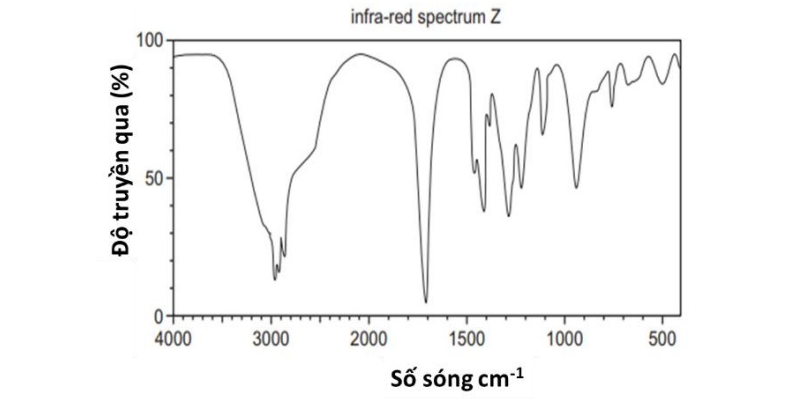
\includegraphics[width=0.6\linewidth]{images_crop_hoa11_de17/ir_spectrum_pentanoic.png}
\end{center}
\choiceTF
{Dựa vào quang phổ IR xác định có nhóm chức \ce{-COOH} của (A)}
{Phổ MS sẽ xác định được khối lượng của chất V thu được từ thí nghiệm trên}
{Phản ứng của chất A với methanol tạo thành chất V là phản ứng thuận nghịch}
{Dựa vào quang phổ IR có thể xác định được công thức phân tử của một hợp chất hữu cơ}
\end{ex}

\bigskip
\noindent\textbf{\large PHẦN III. Câu trắc nghiệm yêu cầu trả lời ngắn.}
\textit{Thí sinh trả lời từ câu 1 đến câu 6.}
\vspace{0.2cm}

\begin{ex}
Cho các chất sau: \ce{CH3-CH2-CHO} (1), \ce{CH2=CH-CHO} (2), \ce{(CH3)2CH-CHO} (3), \ce{CH2=CH-CH2-OH} (4). Chất phản ứng hoàn toàn với lượng dư [H] cùng tạo ra \ce{CH3-CH2-CH2-OH} là bao nhiêu chất?
\vspace{0.8cm}
\end{ex}

\begin{ex}
Cho các tác nhân phản ứng: (a) \ce{H2/Pd}, $t^\circ$; (b) \ce{LiAlH4}; (c) \ce{NaBH4}; (d) dung dịch bromine. Có bao nhiêu tác nhân ở trên có thể chuyển hóa RCHO thành \ce{RCH2OH}?
\vspace{0.8cm}
\end{ex}

\begin{ex}
Cho các phát biểu sau:
\begin{enumerate}[(1)]
  \item Aldehyde phản ứng được với nước bromine.
  \item Ketone không phản ứng được với \ce{Cu(OH)2/OH^-}.
  \item Aldehyde tác dụng với dung dịch \ce{AgNO3/NH3} tạo ra bạc.
  \item Trong các hợp chất carbonyl, chỉ aldehyde bị khử bởi \ce{NaBH4}.
\end{enumerate}
Số phát biểu đúng là bao nhiêu?
\vspace{0.8cm}
\end{ex}

\begin{ex}
Để điều chế \ce{CH3CHO} từ \ce{Al4C3} cần ít nhất bao nhiêu phương trình phản ứng?
\vspace{0.8cm}
\end{ex}

\begin{ex}
Quế có vị cay, mùi thơm nồng, được sử dụng phổ biến làm gia vị, vị thuốc trong Đông y. Hợp chất hữu cơ cinnamaldehyde tạo mùi đặc trưng của quế. Trong phân tử cinnamaldehyde chứa vòng benzene có một nhóm thế. Cinnamaldehyde bị oxi hóa bởi thuốc thử Tollens và có đồng phân hình học dạng trans. Công thức cấu tạo của cinnamaldehyde là:
\begin{center}
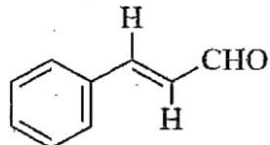
\includegraphics[width=0.28\linewidth]{images_crop_hoa11_de17/cinnamaldehyde_trans.png}
\end{center}
Phân tử khối của cinnamaldehyde là bao nhiêu?
\vspace{0.8cm}
\end{ex}

\begin{ex}
Hợp chất hữu cơ X được dùng nhiều trong tổng hợp hữu cơ. Bằng phương pháp phân tích nguyên tố, người ta xác định được X chứa 62,07\% C; 10,34\% H; còn lại là O. Trên phổ MS của X, người ta thấy có peak ion phân tử $[\text{M}^+]$ có giá trị $m/z$ bằng 58. Trên phổ IR của X có một peak trong vùng 2380 -- 2695 cm$^{-1}$ và một peak trong vùng 1740 -- 1685 cm$^{-1}$. Chất X phản ứng với \ce{Cu(OH)2} trong môi trường kiềm để tạo ra kết tủa màu đỏ gạch. Xác định tổng số nhóm \ce{CH2} trong công thức cấu tạo của X.
\vspace{0.8cm}
\end{ex}

\bigskip
\noindent\textbf{\large PHẦN IV. Câu hỏi tự luận.}
\textit{Thí sinh trình bày lời giải chi tiết vào giấy làm bài.}
\vspace{0.2cm}

\begin{ex}
\textbf{(SBT - CTST)} Trong các phản ứng sau đây, phản ứng nào không thể xảy ra? Hoàn thành phương trình hoá học các phản ứng xảy ra.
\begin{enumerate}[a)]
  \item \ce{CH3CH2-CO-CH3 + [O] ->}
  \item \ce{CH3CH2-OH + [O] ->}
  \item \ce{C6H6 + Cl2 ->[{FeBr$_3$, $t^\circ$}]}
  \item \ce{(CH3)2C(OH)-CH2CH3 + [O] ->}
\end{enumerate}

\vspace{0.2cm}
\noindent\dotfill\\[4pt]
\noindent\dotfill\\[4pt]
\noindent\dotfill\\[4pt]
\noindent\dotfill\\[4pt]
\noindent\dotfill
\end{ex}

\begin{ex}
Cho thí nghiệm: Chuẩn độ acetic acid bằng dung dịch sodium hydroxide 0,15 M. Sau khi thực hiện thí nghiệm chuẩn độ này 3 lần, thu được bảng dưới đây:
\begin{center}
\begin{tabular}{|c|c|c|}
\hline
\textbf{Số lần} & \textbf{Thể tích acetic acid (mL)} & \textbf{Thể tích dung dịch \ce{NaOH} cần dùng (mL)} \\ \hline
1 & 6,0 & 20,0 \\ \hline
2 & 6,0 & 19,9 \\ \hline
3 & 6,0 & 20,0 \\ \hline
\end{tabular}
\end{center}
Xác định nồng độ mol của dung dịch acetic acid.

\vspace{0.2cm}
\noindent\dotfill\\[4pt]
\noindent\dotfill\\[4pt]
\noindent\dotfill\\[4pt]
\noindent\dotfill\\[4pt]
\noindent\dotfill
\end{ex}

\bigskip
\begin{center}
\textbf{---------- HẾT ----------}
\end{center}
\end{document}
